\documentclass[a4paper, top=10mm]{article}
%for writing from the top
\usepackage{fullpage}
%for math
\usepackage{amsmath}
\usepackage{mathrsfs}
\usepackage{amsthm}
%for images
\usepackage{graphicx}
%for color
\usepackage{xcolor}
%for title
\title{\textbf{\huge{La fourmie paresseuse}}}
\author{Enigma n\textsuperscript{o}7}
\date{16\textsuperscript{th} June 2026}

\newtheorem*{hint}{Hint}

\addtolength{\voffset}{-2cm}
\addtolength{\textheight}{5cm}


\begin{document}
	\maketitle
	
	\Large
	Une planche de bois de 2 mètres de long est placée verticalement contre un mur.
	Une fourmi grimpe au milieu de la planche et commence à faire une sieste.
	Malheureusement, la planche glisse le long du mur et tombe au sol.
	
	Quelle distance (au centimètre près) la fourmi endormie a-t-elle parcourue ?
	
	\vspace{2cm}
	
	A wooden plank, 2 meters long, is placed vertically against a wall.
	An ant climbs to the middle of the plank and begins a nap.
	Unfortunately, the plank slides down the wall and falls to the ground.
	
	What distance (to the nearest centimeter) did the sleeping ant travel?
	
	\vspace{1cm}
	
	\begin{center}
		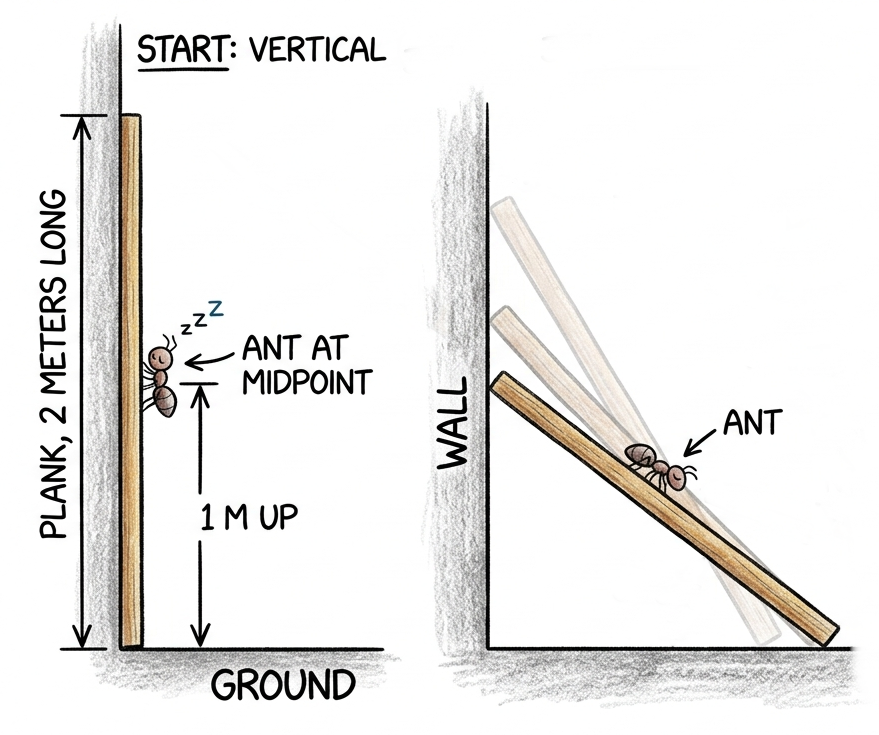
\includegraphics[width=0.8\linewidth]{07ant.png}
	\end{center}
	
	
	% La fourmis decrit un quart de cercle (elle est toujour a egale distance du bas du mur et des cotes de la planche) de rayon 1m.
	% soit 157cm
	
	
\end{document}